\chapter{Motivation}


%===================================================================================================%
\section{Introduction}
%===================================================================================================%


%===================================================================================================%
\section{What is Serverless?}
%===================================================================================================%

"Serverless" is one of the most discussed technologies, prominently featured in many Gartner Hype-Cycle reports that identify trends and emerging technologies which they will think will shape the industries future. 
\autocite{Smith2017Hype2017}
\autocite{Weiss2017Hype2017}
\autocite{Natis2017Hype2017}
\autocite{Walker2017Hype2017}
\autocite{DawsonPhilip2017Hype2017}
Consequently, many asked the question 'what is "serverless"'? Many attempted to define the term but Mike Roberts formulated one of the most universal applicable description:  

\blockquote{\guillemotleft \ ["Serverless" refers to] custom code that's run in ephemeral containers (Function as a Service or "FaaS").[...] Such architectures remove the need for the traditional 'always on' server system sitting behind an application. Depending on the circumstances, such systems can significantly reduce operational cost and complexity. \guillemotright\autocite{Roberts2016ServerlessArchitectures}}

To understand this very broad but commonly accepted definition of "serverless", the first step is to understand what a server is and how a serverless system differs from it. \textquote{A server is a computer designed to process requests and deliver data to another computer over the internet or a local network}\autocite{TheServer}, meaning that a server poses as an accessible endpoint that waits for requests from clients and responds to them. It is \textit{continuously} running, even if there is no task to be processed in order to be ready for incoming requests. This waiting-time is called 'idle time' and presents the most significant difference between servers and serverless systems: while the server waits for incoming requests to process them, in a serverless context a computational unit is created for every incoming request.

\begin{figure}[ht]
    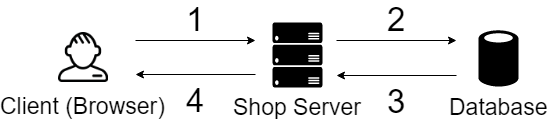
\includegraphics[width=0.9\linewidth]{images/drawio/3tier-oneclient.png}\centering
    \caption {Classic Three-Tier Architecture}
    \label{fig:3tier1client}
\end{figure}

Figure \ref{fig:3tier1client} presents this structure using the example of an online shop. It depicts the classic three-tier-model that consists of the presentation (client), logic (server) and data (database) tier.\autocite{Ramirez2000Three-TierArchitecture} In a situation where a customer intends to purchase an item, first, the client sends a request to the shop's server, which will process it by querying the database for the amount of items in stock, performing the purchase (writing to the database) and lastly responding to the client whether his request was successful or not. More abstract speaking, the action of buying one item is realized as a sequence of a finite amount of steps that have to be passed in order to achieve the desired result. This workflow is the same for each request, but what happens if multiple customers want to $buy$ an item simultaneously? \\
% As illustrated in Figure \ref{fig:3tierNclient}, the amount of steps that have to be performed concurrently to process every request in a timely manner grows with every added client. \\
% \begin{figure}[ht]
%     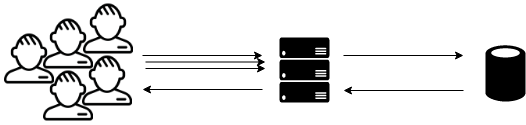
\includegraphics[width=0.9\linewidth]{images/drawio/3tier-multipleclient.png}\centering
%     \caption {Classic Three-Tier Architecture with multiple Clients}
%     \label{fig:3tierNclient}
% \end{figure}
The amount of steps that have to be performed concurrently to process every request in a timely manner grows with every added client but since a server operates on a finite amount of resources, eventually a performance-wise degradation of service occurs. Traditionally, more servers and therefore more available computing power would be added to a system to cope with this challenge. However, this approach results in a very inflexible provision of resources which is illustrated in Figure \ref{graph:provisionedComputePowerServer}. To further support this hypothesis the following section assumes that each server can handle exactly 1000 clients. If 1001 clients simultaneously connect to the system, at least two servers have to be running to satisfy the calls. This directly means that it is never possible to accurately provision just the right amount of processing power for the incoming request but either too much or not enough. 

\begin{figure}[ht]
    \begin{tikzpicture}
        \begin{axis}[
                ,xlabel         = $\# Requests$
                ,ylabel         = {$Provisioned \, Compute \, Power$}
                ,yticklabels    = {,,}
                ,xticklabels    = {,,}
                ,axis x line    = bottom
                ,axis y line    = left
                ,domain         = 0:6
                ,ymajorgrids    = true
                ,grid style     = dashed
                ]
            \addplot [const plot, no marks, color=blue] coordinates {(0,1) (1,2) (2,3) (3,4) (4,5) (5,6)};
            \addplot [color=white]{x};
        \end{axis}
    \end{tikzpicture}\centering
    \caption {Provisioned Compute Power: Server Model}
    \label{graph:provisionedComputePowerServer}
\end{figure}

Comparatively in a serverless approach, the function that executes the steps necessary to fulfill the request is initiated with its own small runtime. How this works from a technical perspective is discussed later on in chapter \ref{sec:serverless} on page \pageref{sec:serverless}. A drastically simplified sketch of this approach can be seen in Figure \ref{fig:serverlessArchHighlevel}. The gateway is an API endpoint that reroutes incoming requests to a server, or in this case to a serverless function that is in turn instantiated. \autocite{Kelly2010UsingInvalidation} This gateway distributes the calls to the newly spun-up functions which is called "fan-out"\autocite{Do2013Limplock}, a term that describes how the system structure fans out after the gateway. 

\begin{figure}[ht]
    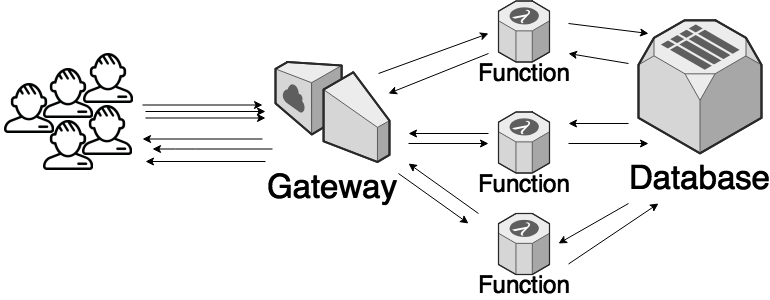
\includegraphics[width=\linewidth]{images/drawio/lambda.png}\centering
    \caption {Serverless Architecture (simplified)}
    \label{fig:serverlessArchHighlevel}
\end{figure}

Since the amount of running functions is directly proportional to the number of incoming requests, the system always provisions the exact processing power needed to sufficiently handle the load. In comparison, a serverless strategy is more efficient, which can be seen in Figure \ref{graph:provisionedComputePowerComparison}.

\begin{figure}[ht]
    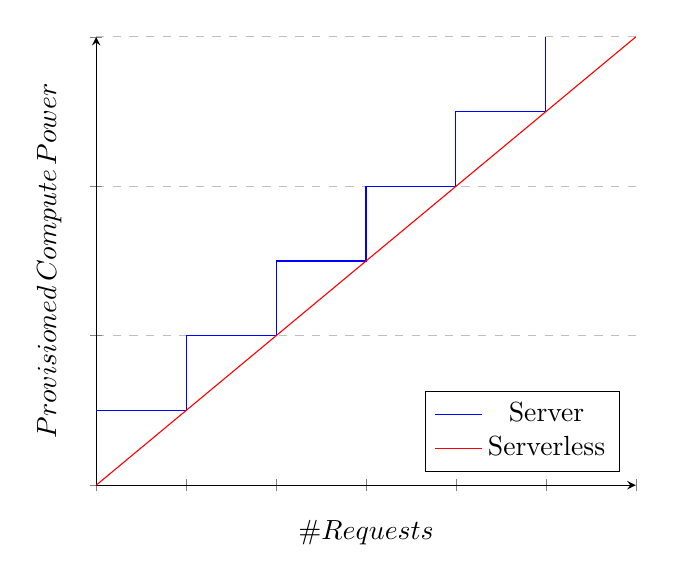
\begin{tikzpicture}
        \begin{axis}[
                ,xlabel         = $\# Requests$
                ,ylabel         = {$Provisioned \, Compute \, Power$}
                ,yticklabels    = {,,}
                ,xticklabels    = {,,}
                ,axis x line    = bottom
                ,axis y line    = left
                ,domain         = 0:6
                ,legend pos     = south east
                ,ymajorgrids    = true
                ,grid style     = dashed
                ]
            \addplot [const plot, no marks, color=blue] coordinates {(0,1) (1,2) (2,3) (3,4) (4,5) (5,6)};
            \addlegendentry{Server}
            \addplot [color=red]{x};
            \addlegendentry{Serverless}
        \end{axis}
    \end{tikzpicture}\centering
    \caption {Provisioned Compute Power Comparison: Server/Serverless}
    \label{graph:provisionedComputePowerComparison}
\end{figure}



%===================================================================================================%
\section{Why Serverless?}
%===================================================================================================%


In recent years \acf{IoT} has been one of the major growth markets and is expected to reach a global revenue of \$457B by the end of 2020, attaining a \acf{CAGR} of 28.5\% over four years.\autocite{Columbus20172017Forecasts} Looking at the most common use cases for IoT applications, it is clear that the prevailing real-life scenarios can be characterized by ubiquitous sensors numbering in the millions or even billions constantly monitoring physical objects, events and humans alike. Right now, these observations are often communicated to a cloud data center for various analyses that in turn trigger reactions to the observed events which aims to improve the efficiency and reliability of the systems and generate valuable insights.\autocite{Yannuzzi2014KeyComputing} \\
This pattern results in a closed-loop \acf{OODA} cycle, where the three major components of the three-tier-model are the information \textit{producers} (sensors), the \textit{cloud endpoint} and the \textit{consumer} or \textit{processor}.\autocite{Shukla2017BenchmarkingApplications} Especially this closed-loop characteristic of IoT applications is essential for their effective use and a low latency between observing events and processing them is therefore a fundamental requirement. To derive actionable insights that have a business impact it is essential to process the data ingress in near real-time since information often has a time-to-live and are only valid for a short amount of time, hence a rapidly scaling processor-concept that is performant enough to digest the data ingress is an imperative system component. \acf{ESP} approaches are an obvious solution to this challenge and all reference IoT solutions from cloud providers \footnote{\url{https://aws.amazon.com/iot-core/features/}}\textsuperscript{,}\footnote{\url{https://microsoft.com/en-in/cloud-platform}} include some element of event streaming.


%===================================================================================================%
\section{Scientific Body of Knowledge}
%===================================================================================================% 

Academically speaking, serverless architectures have been a topic of interest for several years. The vast majority of research, however, is focussing on defining the technology and is contend with describing and characterizing it. Eight most important scientific publications on the topic of serverless where made in major journals:  Baldini\autocite{Baldini2017TheComputing}, McGrath\autocite{McGrath2017ServerlessPerformance}, Nastic\autocite{Nastic2017AComputingb}, Malawski\autocite{Malawski2017ServerlessFunctions}, Castro\autocite{Castro2017ServerlessService}, Ellis\autocite{Ellis2017FunctionsDocker}, Bila\autocite{Bila2017LeveragingContainers} and Stigler\autocite{Stigler2018UnderstandingComputing}.\\

\begin{enumerate}
    \item 
        \textbf{Baldini et. al.} describe "serverless" as \blockquote{a set of stateless functions, along with the events that should trigger their activation [and] a serverless runtime [that] allocates resources as events arrive, avoiding the need for costly pre-allocated or dedicated hardware.} They discuss the challenges that emerge when programming a composition of functions, where the composition is a serverless function itself. Moreover, they identify three main constraints for composing functions: First, functions should be considered as black boxes, secondly, function composition should obey a substitution principle with respect to synchronous invocation and third,  invocations should not be billed two times. As a result, they demonstrate an addition to the core of an open-source serverless runtime that enables composition of functions that satisfies all three constraints.\autocite{Baldini2017TheComputing}
    \item
        \textbf{McGrath and Brenner} discuss the design, implementation and operation of a performance-oriented serverless computing platform implemented in. NET that utilizes Windows containers as function execution environments and is deployed on Microsoft Azure. They focus on implementation obstacles such as scaling and container recovery. Furthermore, they propose metrics to measure the performance of serverless plattforms like AWS Lambda, Azure Functions, Google Cloud Functions and Apache OpenWhisk and compare their prototypical function to the test results from commercial serverless platforms. Overall, they observe a higher throughput with their prototype in comparison.
    \item
        \textbf{Nastic et. al.} apply the the serverless architecture pattern to the challenge of edge-data analytics 
\end{enumerate}



Interestingly they all share some common characteristics: they focus on \textit{how} to implement serverless architecture or \textit{what} it is but do not conduct any extensive comparative analysis aiming to directly study the differences to other architectural patterns. Equally striking is the fact, that every study was published in 2017 or even 2018 although the first widespread public service offering serverless computing, AWS Lambda, was introduced back in 2014.\autocite{Lindblom2014AWSBlog}\\


The scientific body of knowledge and the academic understanding of the topic will be further examined in chapter \ref{sec:serverless}.

%===================================================================================================%
\section{Research Objective}
%===================================================================================================%


The purpose of this research is to evaluate the suitability and viability of the serverless architecture pattern by comparing it in a prototypical scenario. The result will be a simplified decision-framework for architects that enables them to decide if a "serverless" architectural approach is fitted for their stream-processing use-case.

One sub-objective is to asses the current industry understanding of "serverless" and evaluate the suitability and viability of this architecture pattern.
Moreover, it is supposed to assist the process of highlevel system design by providing a reference and guidance by introducing fPaaS\footnote{"Function-Platform-as-a-Service". Defined by Gartner \autocite{Chandrasekaran2017EvolutionWhen}} capabilities and caveats.\\
An important aspect is to discuss not only the advantages of the serverless architecture pattern but also to evaluate the caveats and shortcomings of said architecture and its impact. To provide the reader a comprehensive view on the subject, it is additionally the goal of this research to characterize the design compromises that have to be made when applying the serverless approach.  

%===================================================================================================%
\section{Summary}
%===================================================================================================%